The number of events observed in data and in the Standard model predictions are
reported in \cref{tab:results} for a selected set of exclusive signal regions as
defined in \cref{sec:event-selection-1}.
\begin{table}[!h]
  \centering
  \resizebox{\linewidth}{!}{\begin{tabular}{lccccc}
    \toprule
    \multicolumn{6}{c}{Analysis Results} \\
    \midrule \midrule
    \textbf{Exclusive Signal Region } & EM2 & EM4 & EM6 & EM8 & EM9 \\
    Observed events (36.1~$\ifb$) & 67475 & 27843 & 2975 & 512 & 223 \\
    \midrule
    SM prediction & $67100 \pm 1400$ & $27640 \pm 610$ & $2825 \pm 78$
                  & $463 \pm 19$ & $213 \pm 9$ \B \\ \cline{2-6}
    $\wenuplusjets$    & $5510 \pm 140$ & $1789 \pm 59$ & $147 \pm 9$
                       & $18 \pm 1$ & $8 \pm 1$ \T \\
    $\wmunuplusjets$   & $6120 \pm 200$ & $2021 \pm 82$ & $173 \pm 9$
                       & $21 \pm 5$ & $11 \pm 1$ \\
    $\wtaunuplusjets$  & $13680 \pm 310$ & $4900 \pm 110$ & $397 \pm 11$
                       & $55 \pm 5$ & $29 \pm 2$ \\
    $\zeeplusjets$     & $0.03 \pm 0$ & $0.02 \pm 0.02$ & $0 \pm 0$
                       & $0 \pm 0$ & $0 \pm 0$ \\
    $\zmumuplusjets$   & $167 \pm 8$ & $36 \pm 2$ & $2 \pm 0.2$
                       & $0.4 \pm 0.1$ & $0.5 \pm 0.1$ \\
    $\ztautauplusjets$ & $185 \pm 6$ & $68 \pm 4$ & $5.1 \pm 0.3$
                       & $0.3 \pm 0.1$ & $0.31 \pm 0.04$ \\
    $\znunuplusjets$   & $37600 \pm 970$ & $17070 \pm 460$ & $1933 \pm 57$
                       & $337 \pm 12$ & $153 \pm 7$ \\
    $t \bar{t}$, single top & $2230 \pm 200$ & $848 \pm 86$ & $43 \pm 6$
                            & $4 \pm 1$ & $1.3 \pm 0.4$ \\
    Diboson & $1327 \pm 90$ & $874 \pm 64$ & $124 \pm 16$
            & $26 \pm 5$ & $10 \pm 2$ \\
    Multijet background & $170 \pm 160$ & $13 \pm 13$ & $1 \pm 1$
                        & $1 \pm 1$ & $0.1 \pm 0.1$ \\
    Non-collision background & $71 \pm 71$ & $18 \pm 18$ & $0 \pm 0$
                             & $0 \pm 0$ & $0 \pm 0$ \\
    \bottomrule
  \end{tabular}}
  \caption{Number of events in the observed data and Standard Model predictions
    in a representative set of signal regions as defined in
    \cref{sec:event-selection-1}. For the \gls{sm} predictions the quoted
    uncertainty includes both statistical and systematic uncertainties.}
  \label{tab:results}
\end{table}
\begin{figure}[!th]
  \centering
  \begin{subfigure}[t]{.48\linewidth}
    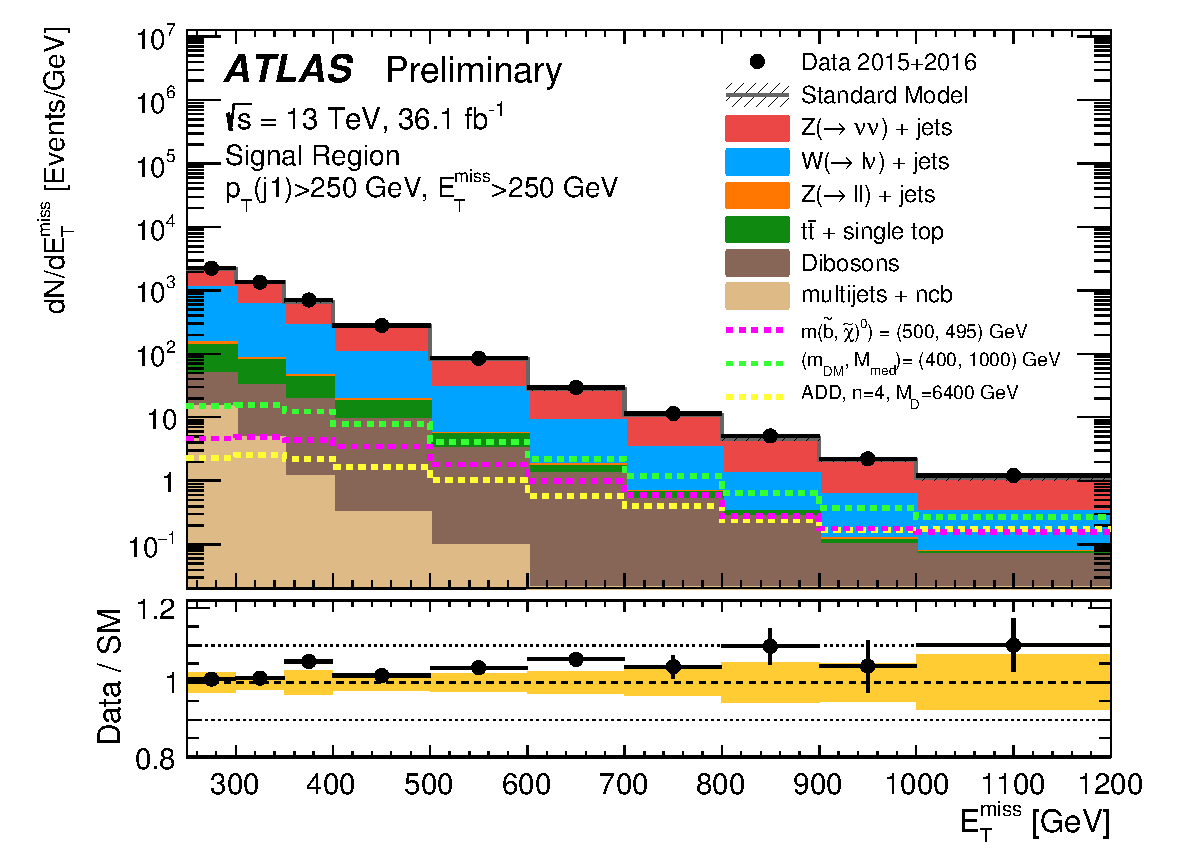
\includegraphics[width=\linewidth]{sr_mod_ind_met}
    \caption{$\met$ distribution.}
    \label{fig:sr_et_miss}
  \end{subfigure}
  \begin{subfigure}[t]{.48\linewidth}
    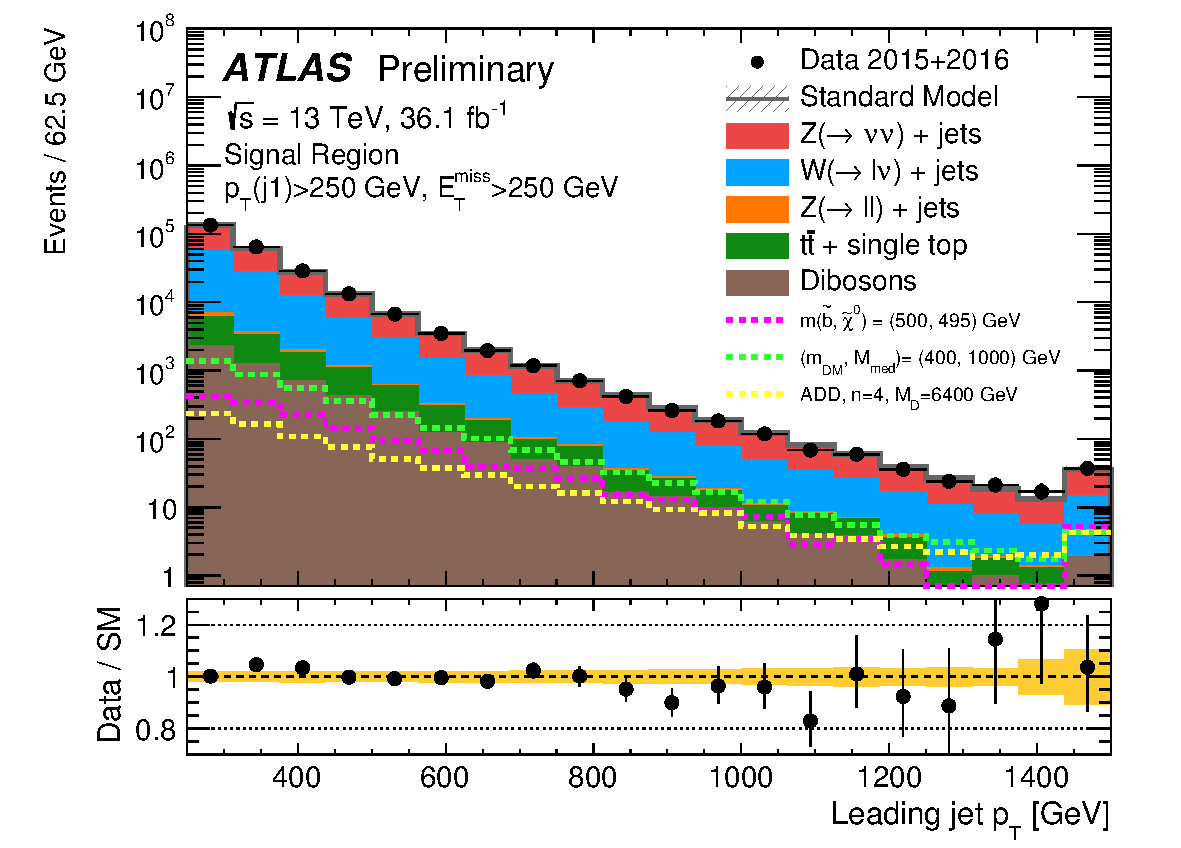
\includegraphics[width=\linewidth]{sr_mod_ind_jetpt}
    \caption{Leading jet $\pt$ distribution.}
    \label{fig:sr_jet1_pt}
  \end{subfigure}
  \caption{Distribution of the $\met$ and the leading jet $\pt$ for IM1 signal
    region compared with the background estimates from the background only fit
    in the control regions. The distributions of different signal models are
    superimposed for comparison. The contribution from the multi-jet and NCB
    background is negligible and not reported in the plot. In the ratio window
    the error bars include experimental and systematic uncertainties.}
  \label{fig:sr_plots}
\end{figure}
\begin{figure}[!th]
  \centering
  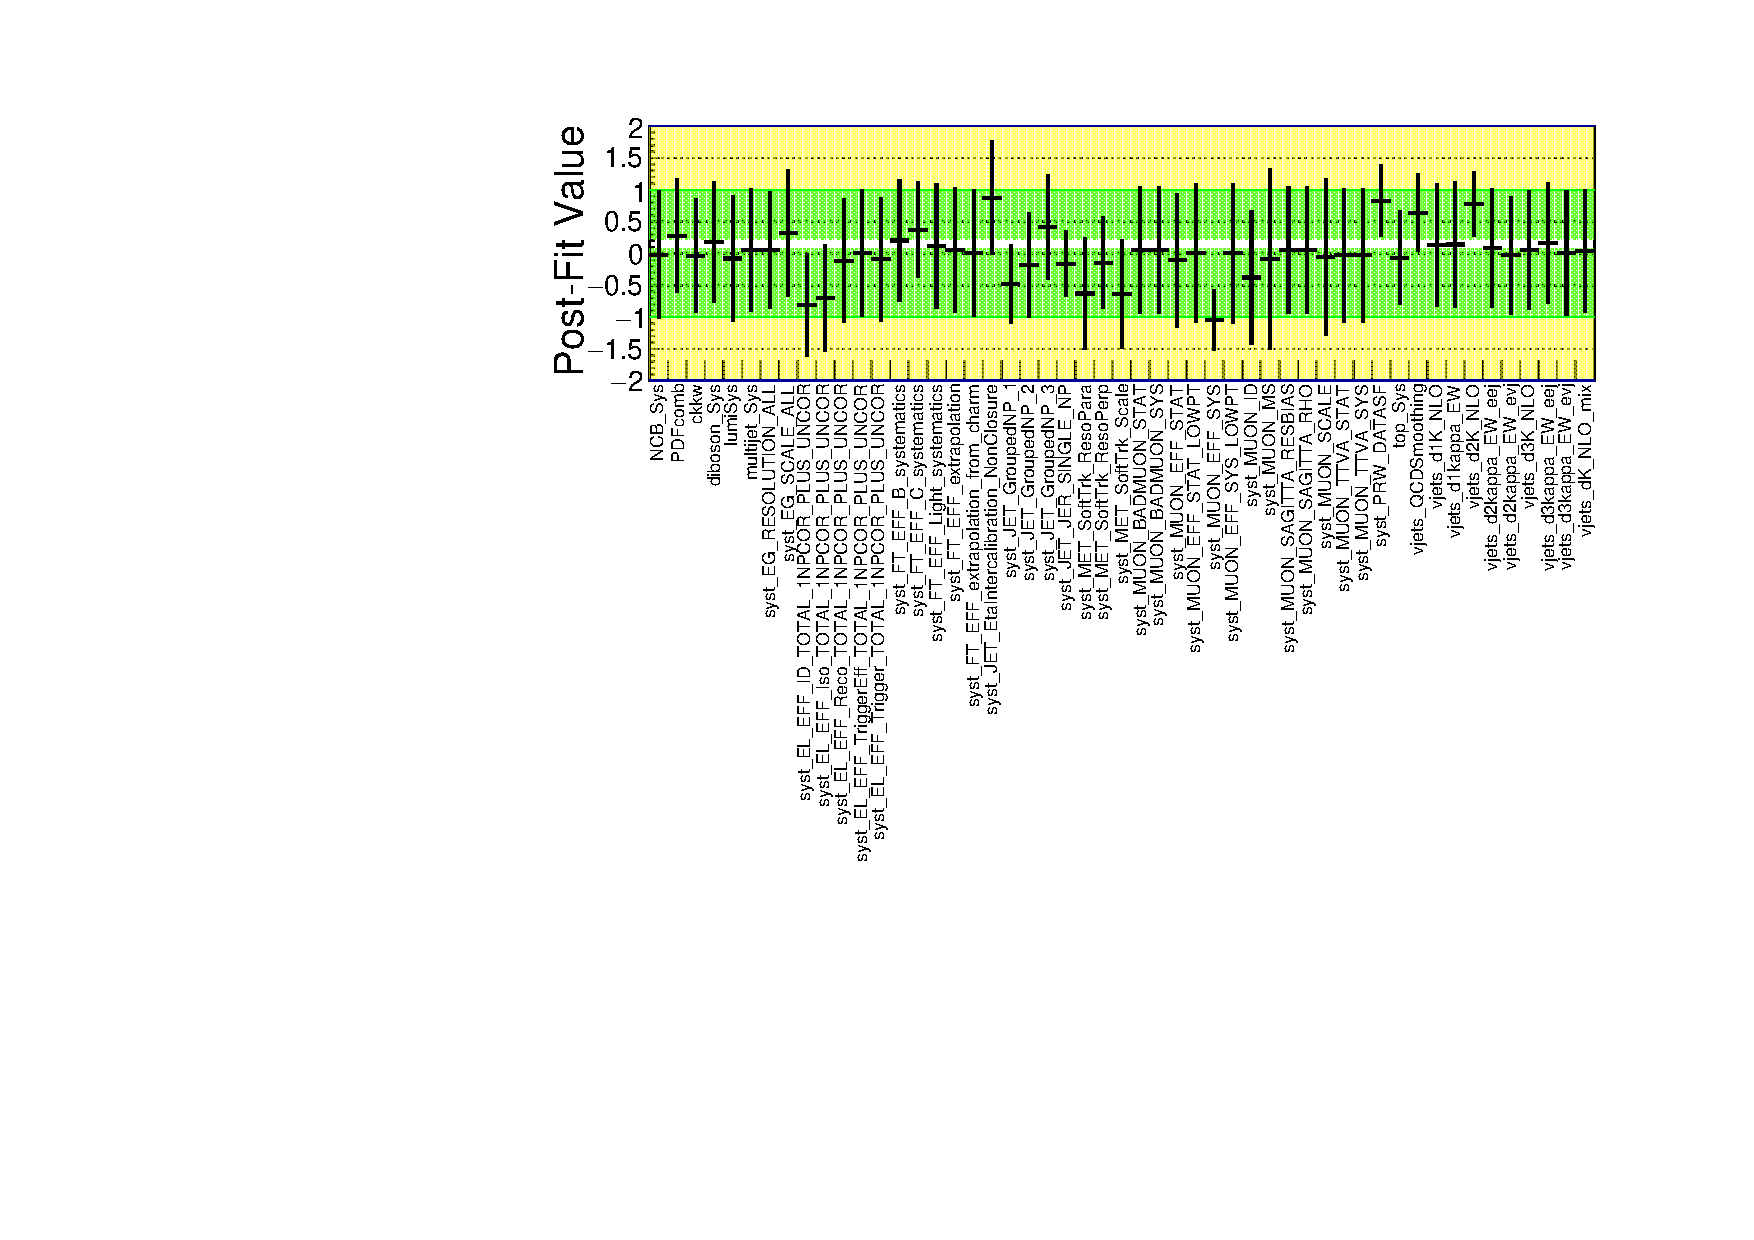
\includegraphics[width=\linewidth]{np_pull_plot}
  \caption{Values of the nuisance parameters used in the analysis after the
    control and signal region inclusive fit to the data.}
  \label{fig:np_pull}
\end{figure}
\begin{figure}[!hb]
  \centering
  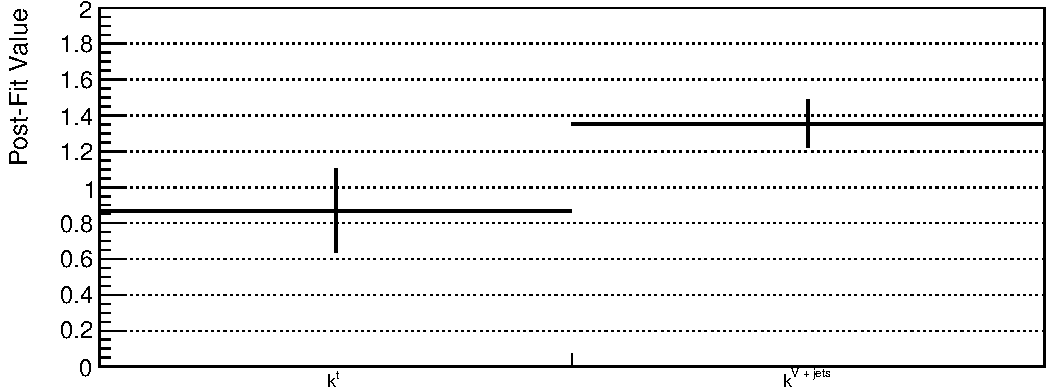
\includegraphics[width=\linewidth]{kfactors}
  \caption{Values of the normalization factors for the V + jets and single top
    backgrounds after the control and signal region inclusive fit to the data.}
  \label{fig:kfactors}
\end{figure}
\begin{figure}[!th]
  \centering
  \begin{subfigure}[t]{.48\linewidth}
    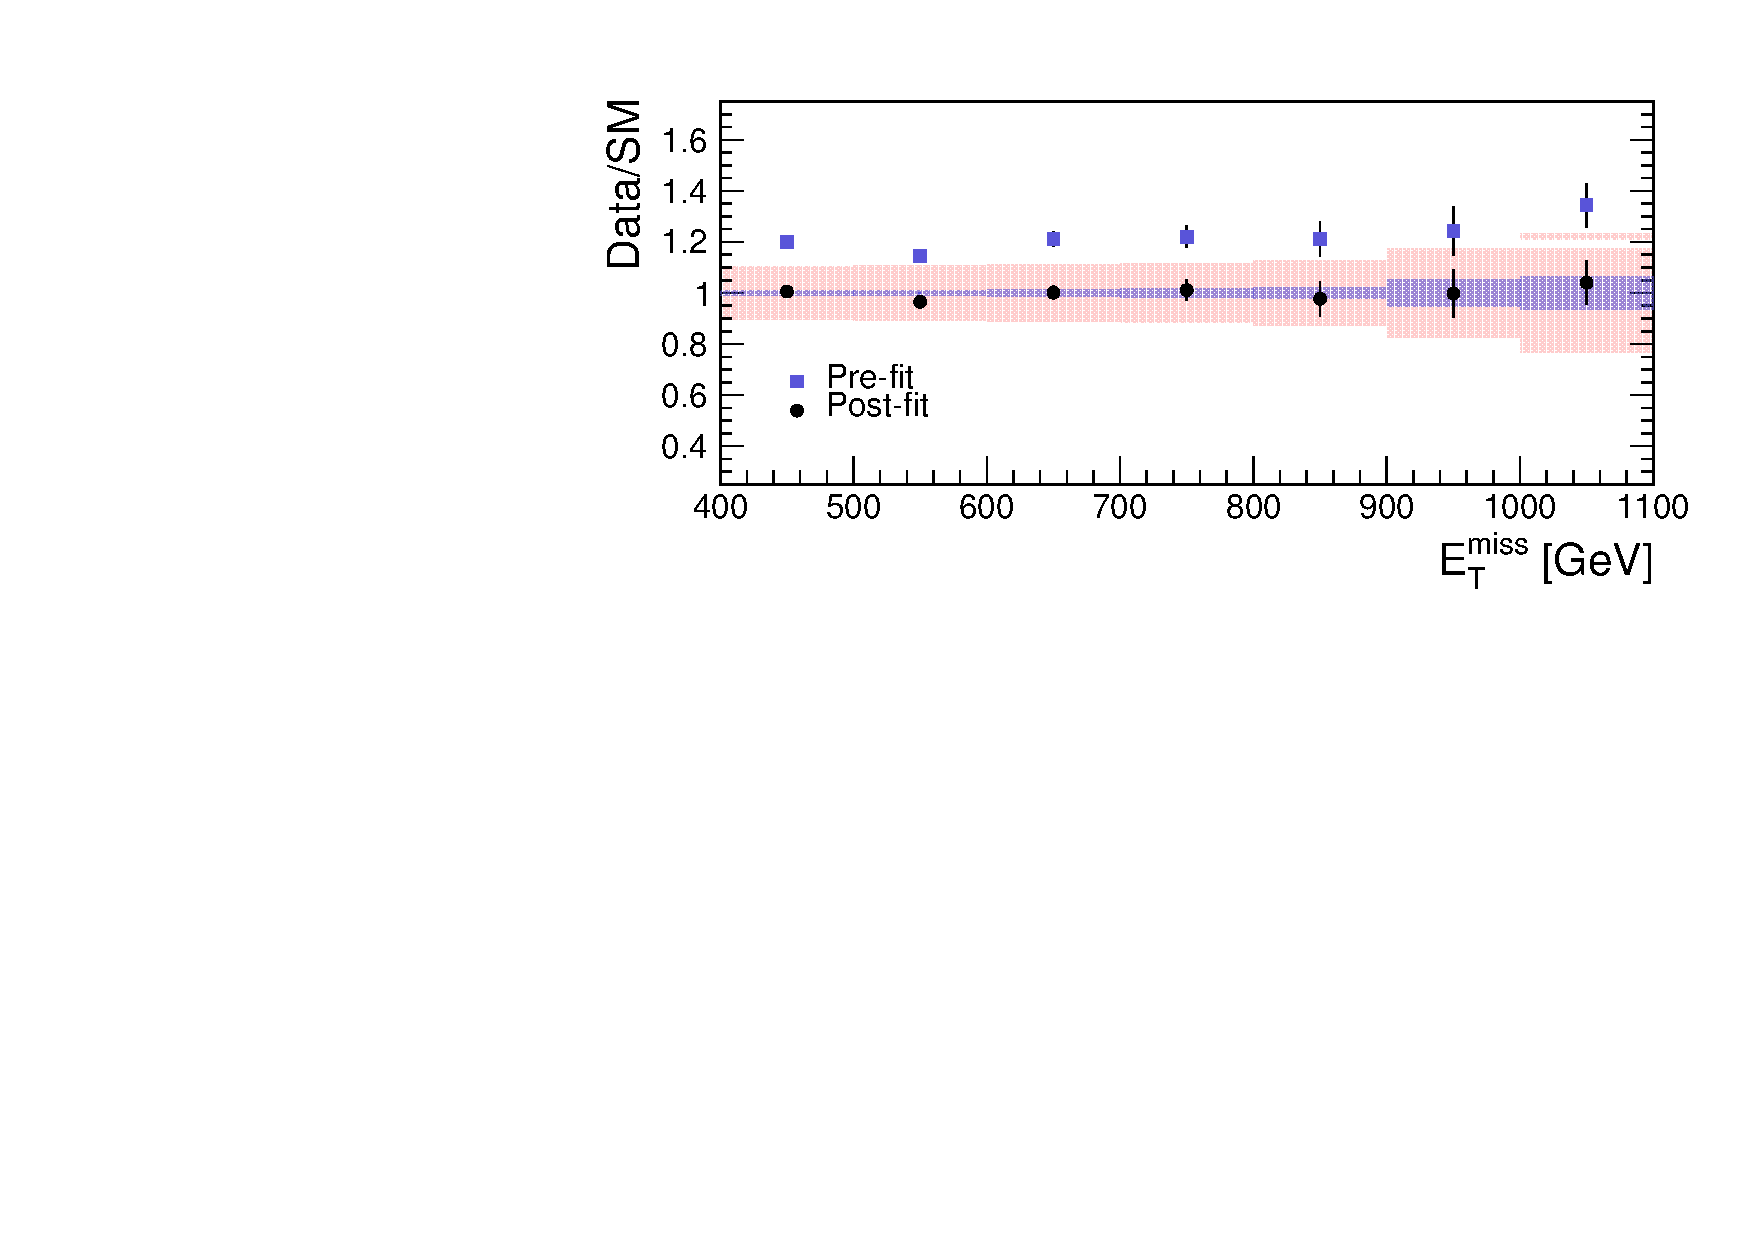
\includegraphics[width=\linewidth]{crele_pull}
    \caption{$\crele$.}
    \label{fig:crele_pull}
  \end{subfigure}
  \begin{subfigure}[t]{.48\linewidth}
    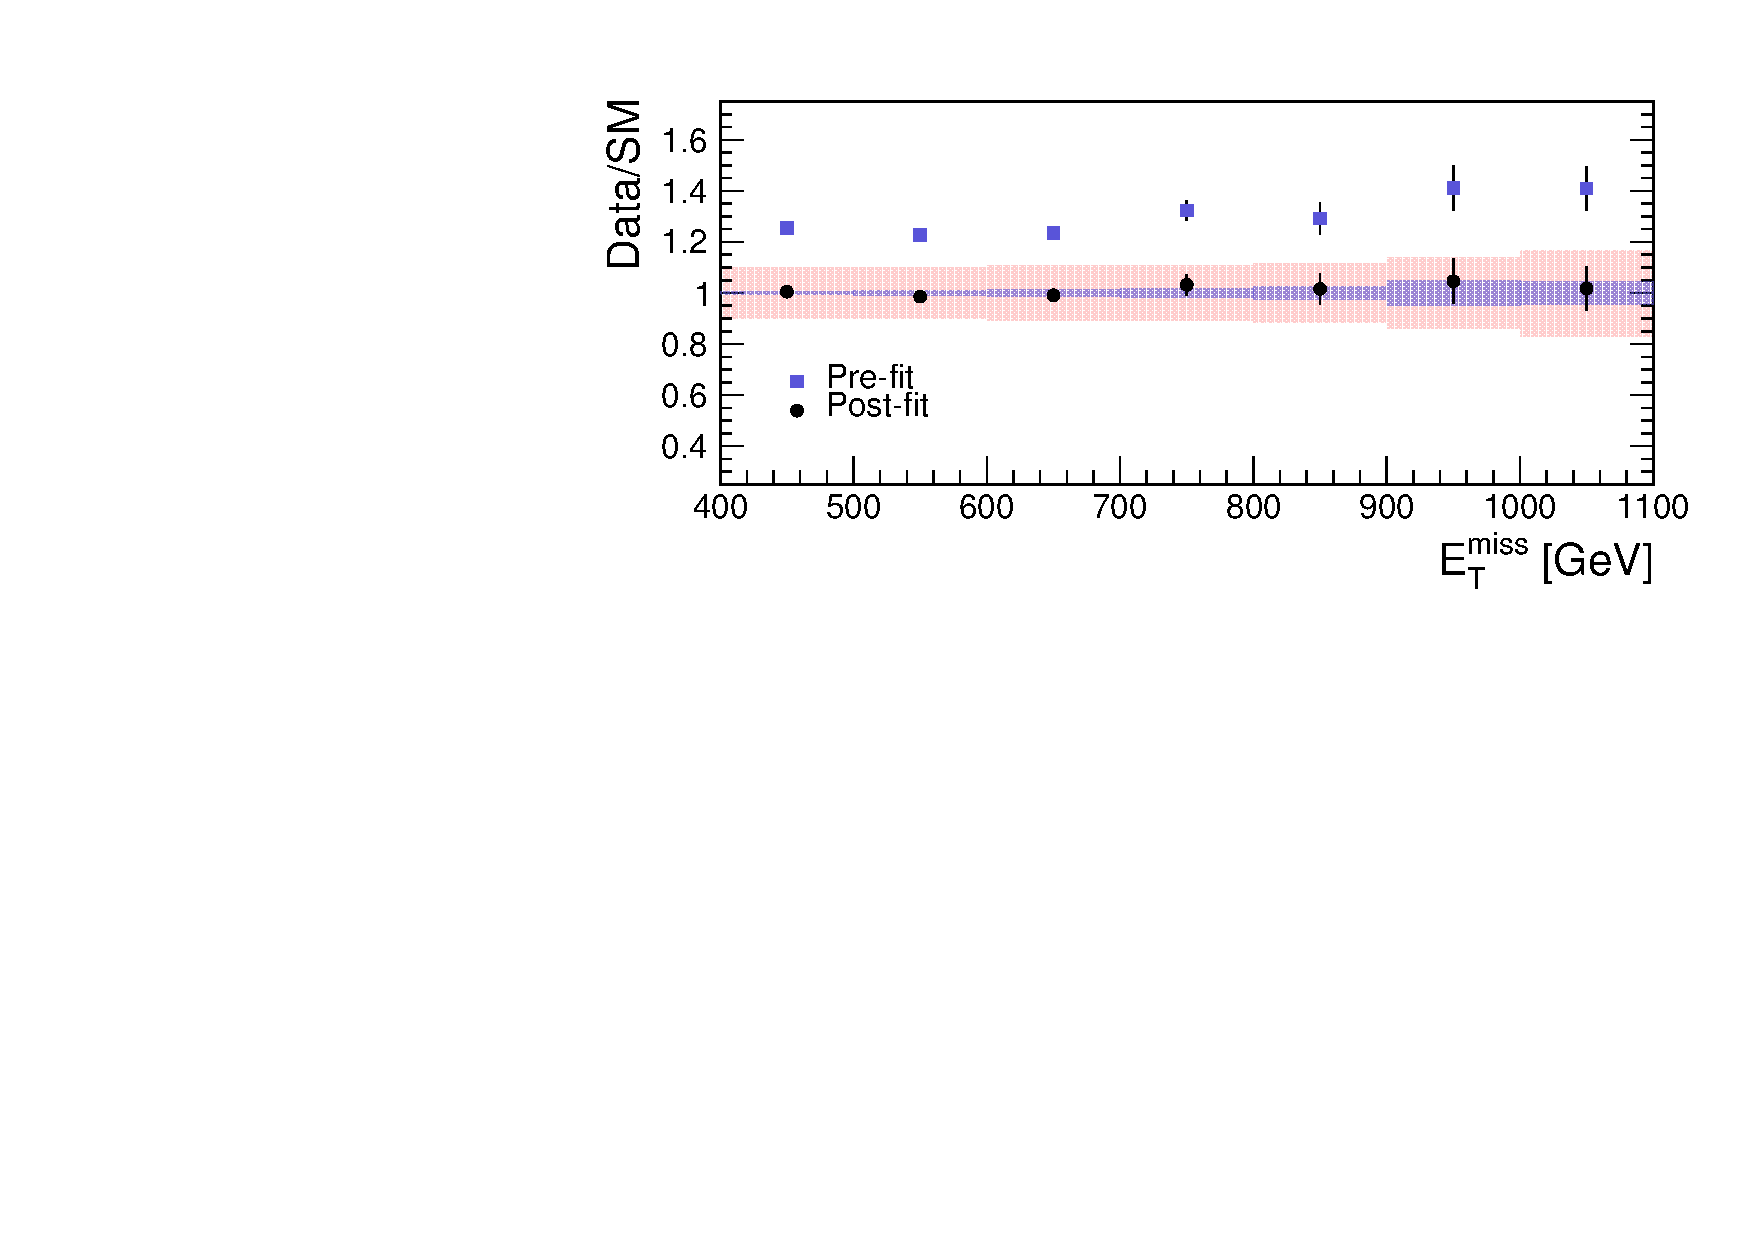
\includegraphics[width=\linewidth]{crwmn_pull}
    \caption{$\crwmn$.}
    \label{fig:crwnm_pull}
  \end{subfigure}
  \begin{subfigure}[t]{.48\linewidth}
    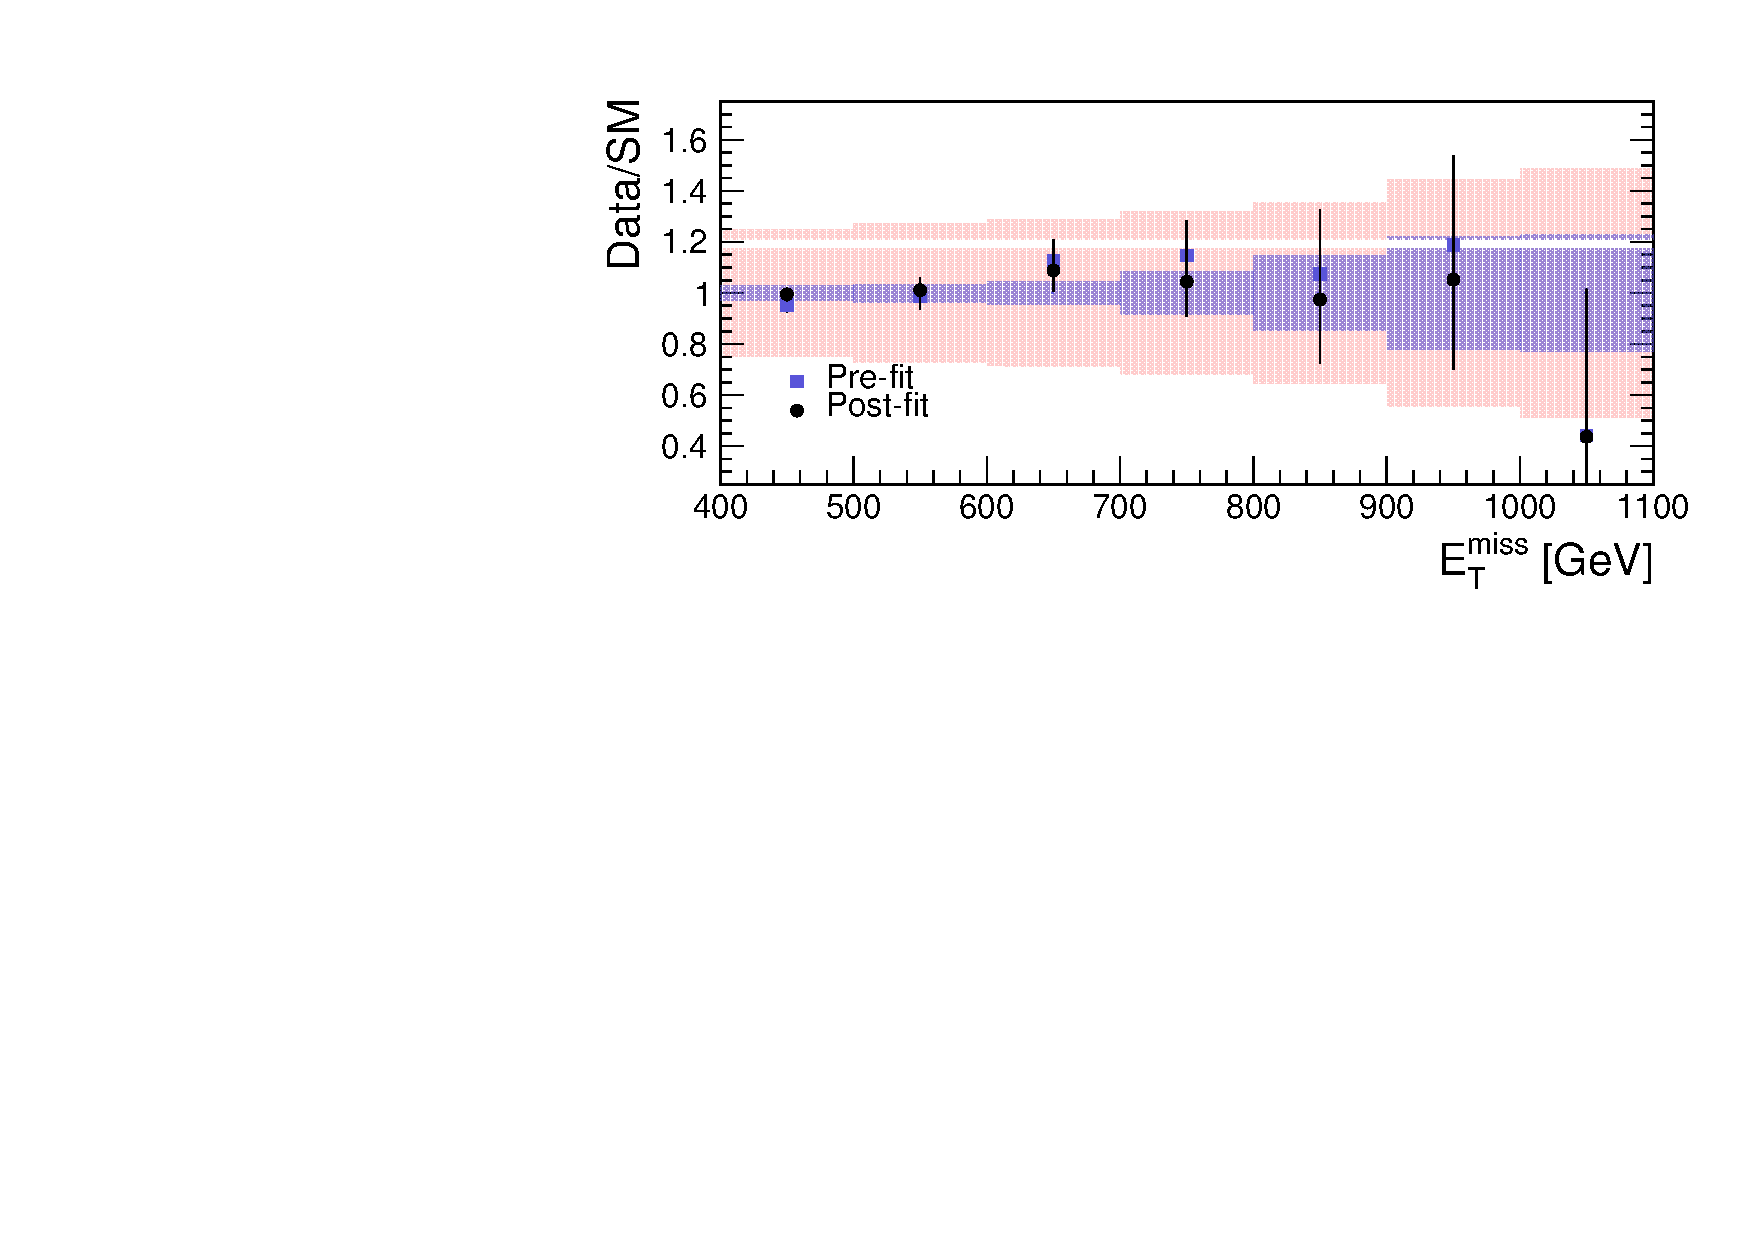
\includegraphics[width=\linewidth]{crtop_pull}
    \caption{$\crtop$.}
    \label{fig:crtop_pull}
  \end{subfigure}
    \begin{subfigure}[t]{.48\linewidth}
    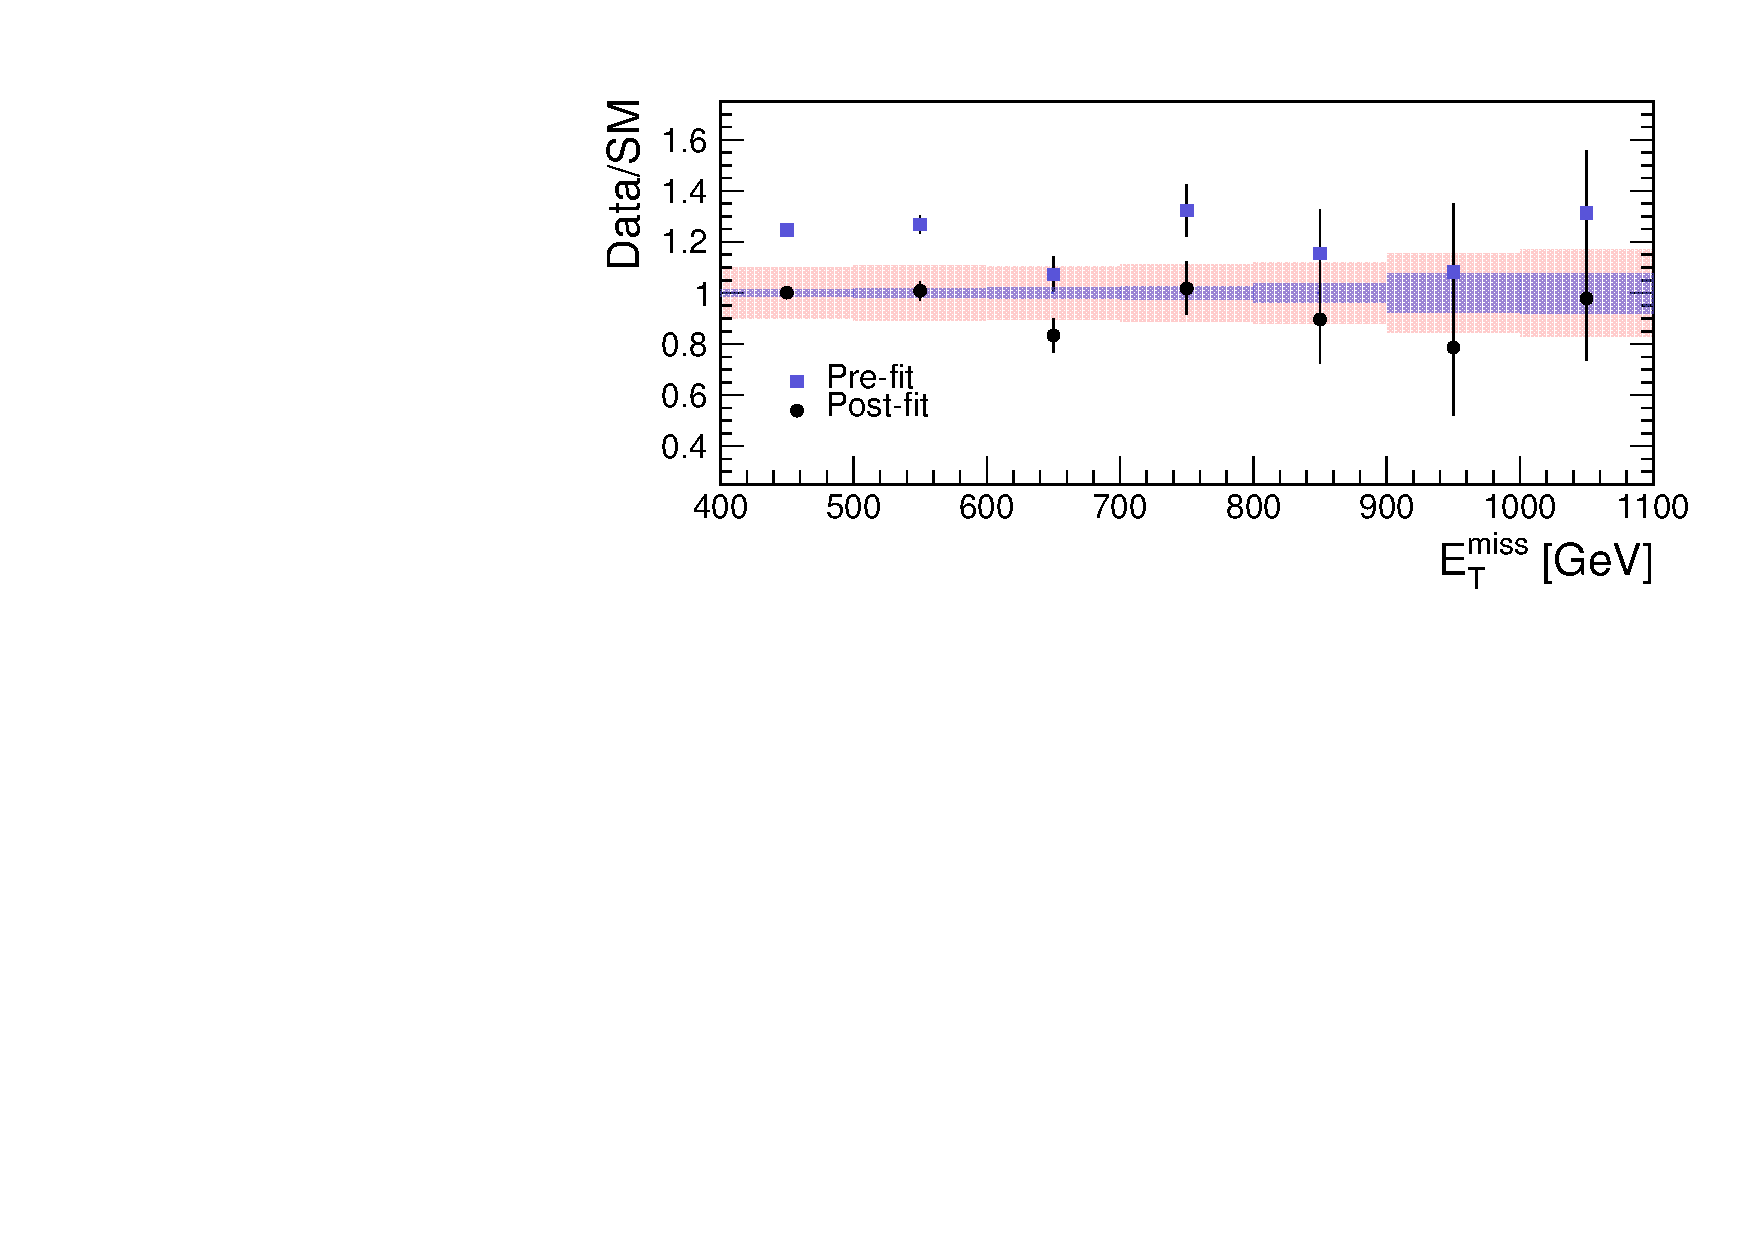
\includegraphics[width=\linewidth]{crzmm_pull}
    \caption{$\crzmm$.}
    \label{fig:crzmm_pull}
  \end{subfigure}
  \begin{subfigure}[t]{.48\linewidth}
    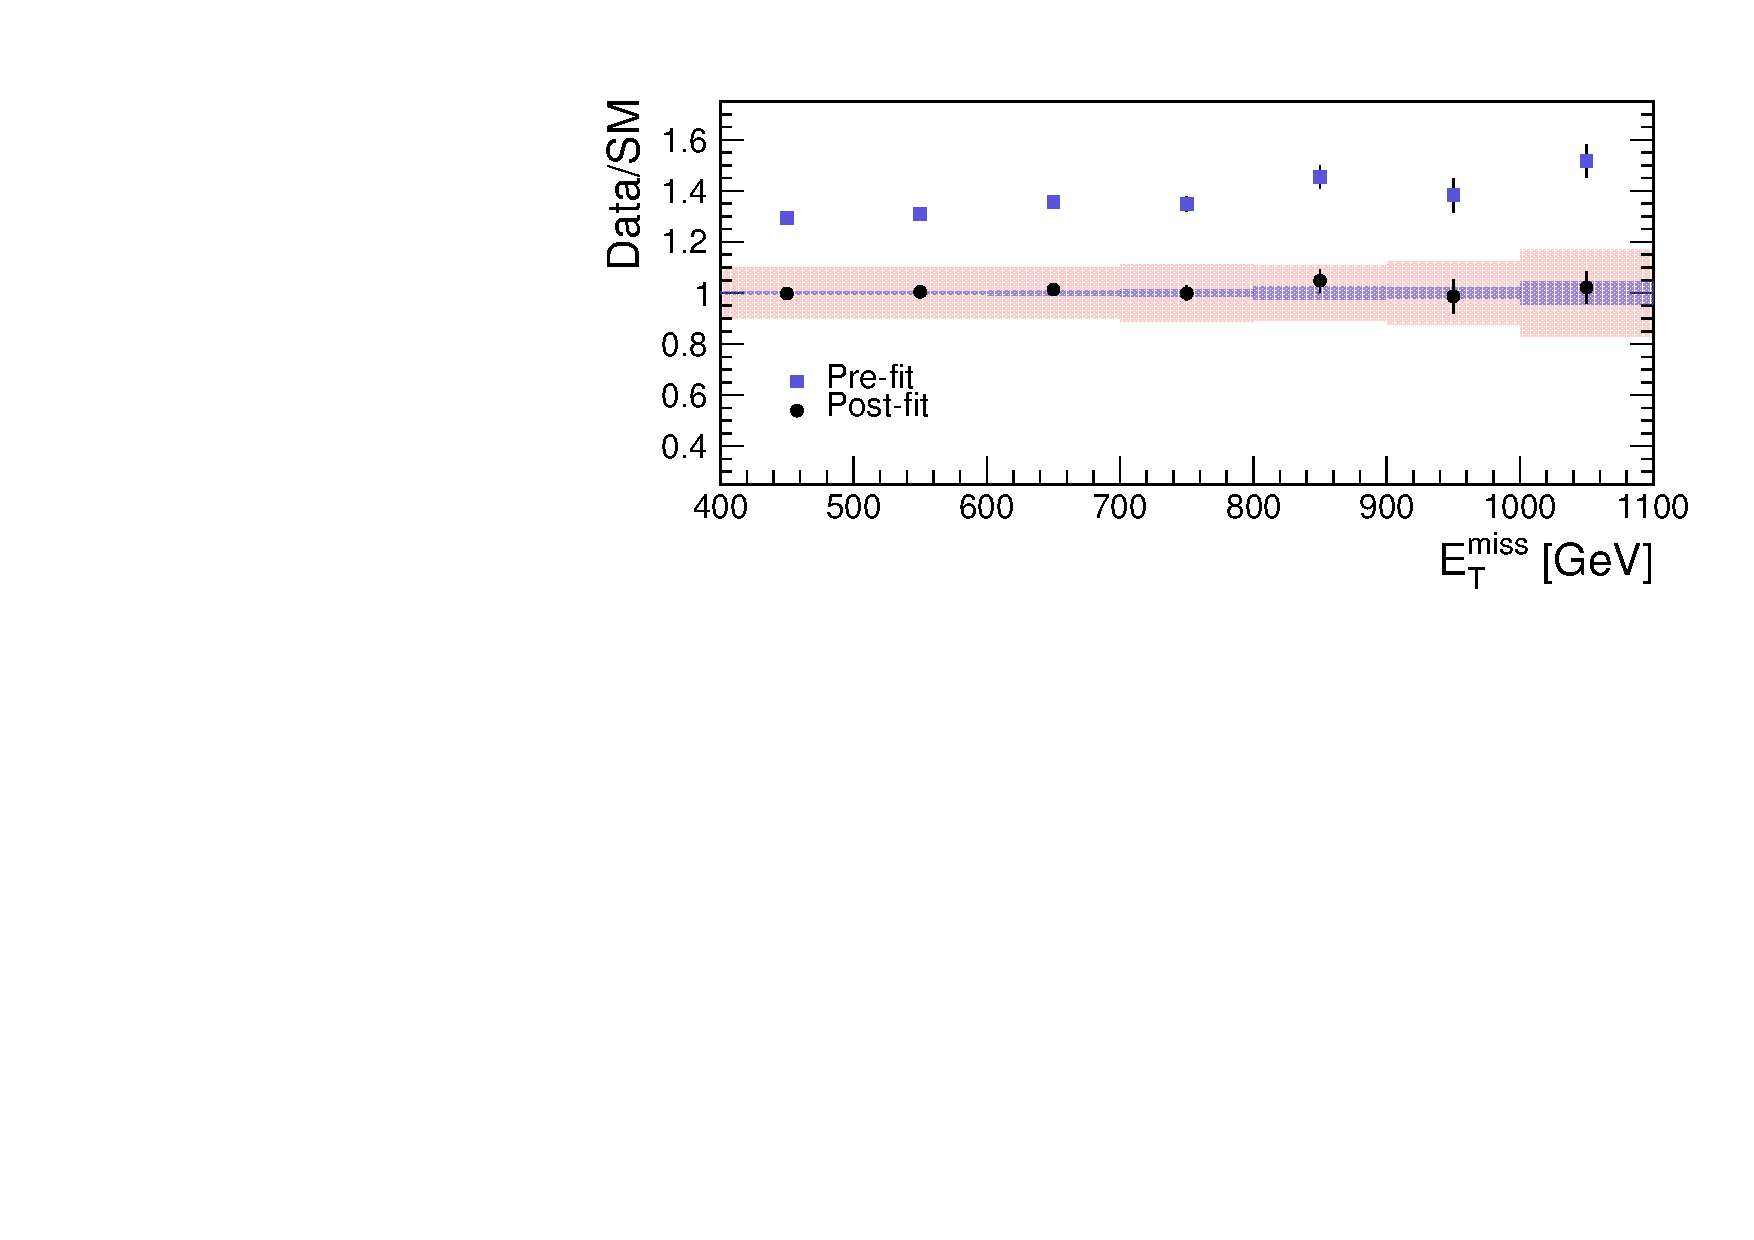
\includegraphics[width=\linewidth]{sr_pull}
    \caption{Signal Region.}
    \label{fig:sr_pull}
  \end{subfigure}
  \caption{Comparison between data and Monte Carlo before and after the fit
    performed separately for each region. The shaded areas represent the pre and
    post-fit total (statistic and systematic) uncertainties on the background
    estimation \note{these shaded areas are set on the value 1 of the bin and
      are a relative error for the pre and post-fit results. I'm not sure I
      understand why they are put on 1 and what are they supposed to mean, maybe
      I'm going to remove them from the plot (sort of Asimov data).}.}
  \label{fig:reagion_pulls}
\end{figure}
%%% Local Variables:
%%% mode: latex
%%% TeX-master: "../search_for_DM_LED_with_ATLAS"
%%% End:
